\section{Tricks}

This section describes random tricks used to speed up rendition. They range from simple precomputed cos/sin tables to what I consider one of the most beautiful hacks in the engine: Linear Feedback Shift Register.




\subsection{Cos/Sin table lookup}
\cw{cos} and \cw{sin} are expensive methods involving floating point calculations. They are extensively used at runtime. To speed things up, the engine generates and caches them in a lookup array (one value per angle) at startup. To save RAM, it exploits a math property ($cos(X) = sin(X + 90)$) to avoid 360 \cw{cos} method calls and 240 bytes of RAM by reusing the \cw{sin} table as follows:\\
\par

\begin{minipage}{\textwidth}
\lstinputlisting[language=C]{code/sin_cos_table.c}
\end{minipage}


\begin{figure}[H]
 \centering
  
\includegraphics[width=\textwidth]{imgs/drawings/cos_sin_table.pdf}
\end{figure}








\subsection{FizzleFade}
While most screen transitions are done with a fade to black (by shifting the palette), there are two instances when the screen transitions via fizzling:
\begin{itemize}
	\item When dying
	\item When killing a boss
\end{itemize}
Below are a series of screenshots to illustrate fizzling. During the transition, each pixel on the screen is turned to red (when dying) or blue (when dispatching a boss). Each pixel is written only once and seemingly at random. 



\begin{minipage}{\textwidth}
\centering
  \scaledimage{.9}{fizzlefade/dying/screenshot_16.png}\\
  \vspace*{0.5cm}
  \scaledimage{.9}{fizzlefade/dying/screenshot_19.png}\\
\end{minipage}

\begin{minipage}{\textwidth}
\centering
  \scaledimage{.9}{fizzlefade/dying/screenshot_52.png} \\
  \vspace*{0.5cm}
  \scaledimage{.9}{fizzlefade/dying/screenshot_86.png} \\
\end{minipage}


\begin{minipage}{\textwidth}
\centering
  \scaledimage{.9}{fizzlefade/boss/screenshot_60.png} \\
  \vspace*{0.5cm}
  \scaledimage{.9}{fizzlefade/boss/screenshot_66.png}  \\
\end{minipage}

\begin{minipage}{\textwidth}
\centering
  \scaledimage{.9}{fizzlefade/boss/screenshot_102.png}\\
\vspace*{0.5cm}
  \scaledimage{.9}{fizzlefade/boss/screenshot_130.png}\\
\end{minipage}

To implement this effect, a naive approach would have been to use the pseudo random generator \cw{US\_RndT} and keep track of which pixels had been fizzled. However, this would make the fade non-deterministic with regard to duration and would also waste CPU cycles since the same pixel coordinates (X,Y) could come up several times. There is a much faster and more elegant way to implement a pseudo-random value generator. The code responsible for this effect can be found in \cw{id\_vh.cpp}, function \cw{FizzleFade}. At first, it is not obvious how it works.\\
\par
\begin{minipage}{\textwidth}
\lstinputlisting[language=C]{code/fizzlefade.c}
\end{minipage}
\par
Which can be read as:\\
\begin{itemize}
\item Initialize \cw{rndval} to 1.
\item Break it down in 8 + 7 bits: use 8 bits to generate a X coordinate and 7 bits for a Y coordinate. Turn this pixel to red.
\item Subject \cw{rndval} to a soup of XORing.
\item When \cw{rndval} value is somehow back to 1: Stop.
\end{itemize}        
This feels like dark magic. How is \cw{rndval} supposed to return to value 1? That technique is called Linear Feedback Shift Register. The idea is to use one register to store a state, generate the next state, and also generate a value. To get the next value, you do a right shift. Since the rightmost bit disappears, a new one to the left is needed. To generate this new bit, the register uses "taps" which are bit offsets used to XOR together values and generate the new bit value. A Fibonnaci representation shows a simple LFSR with two taps.\\
\par

\begin{figure}[H]
 \centering
  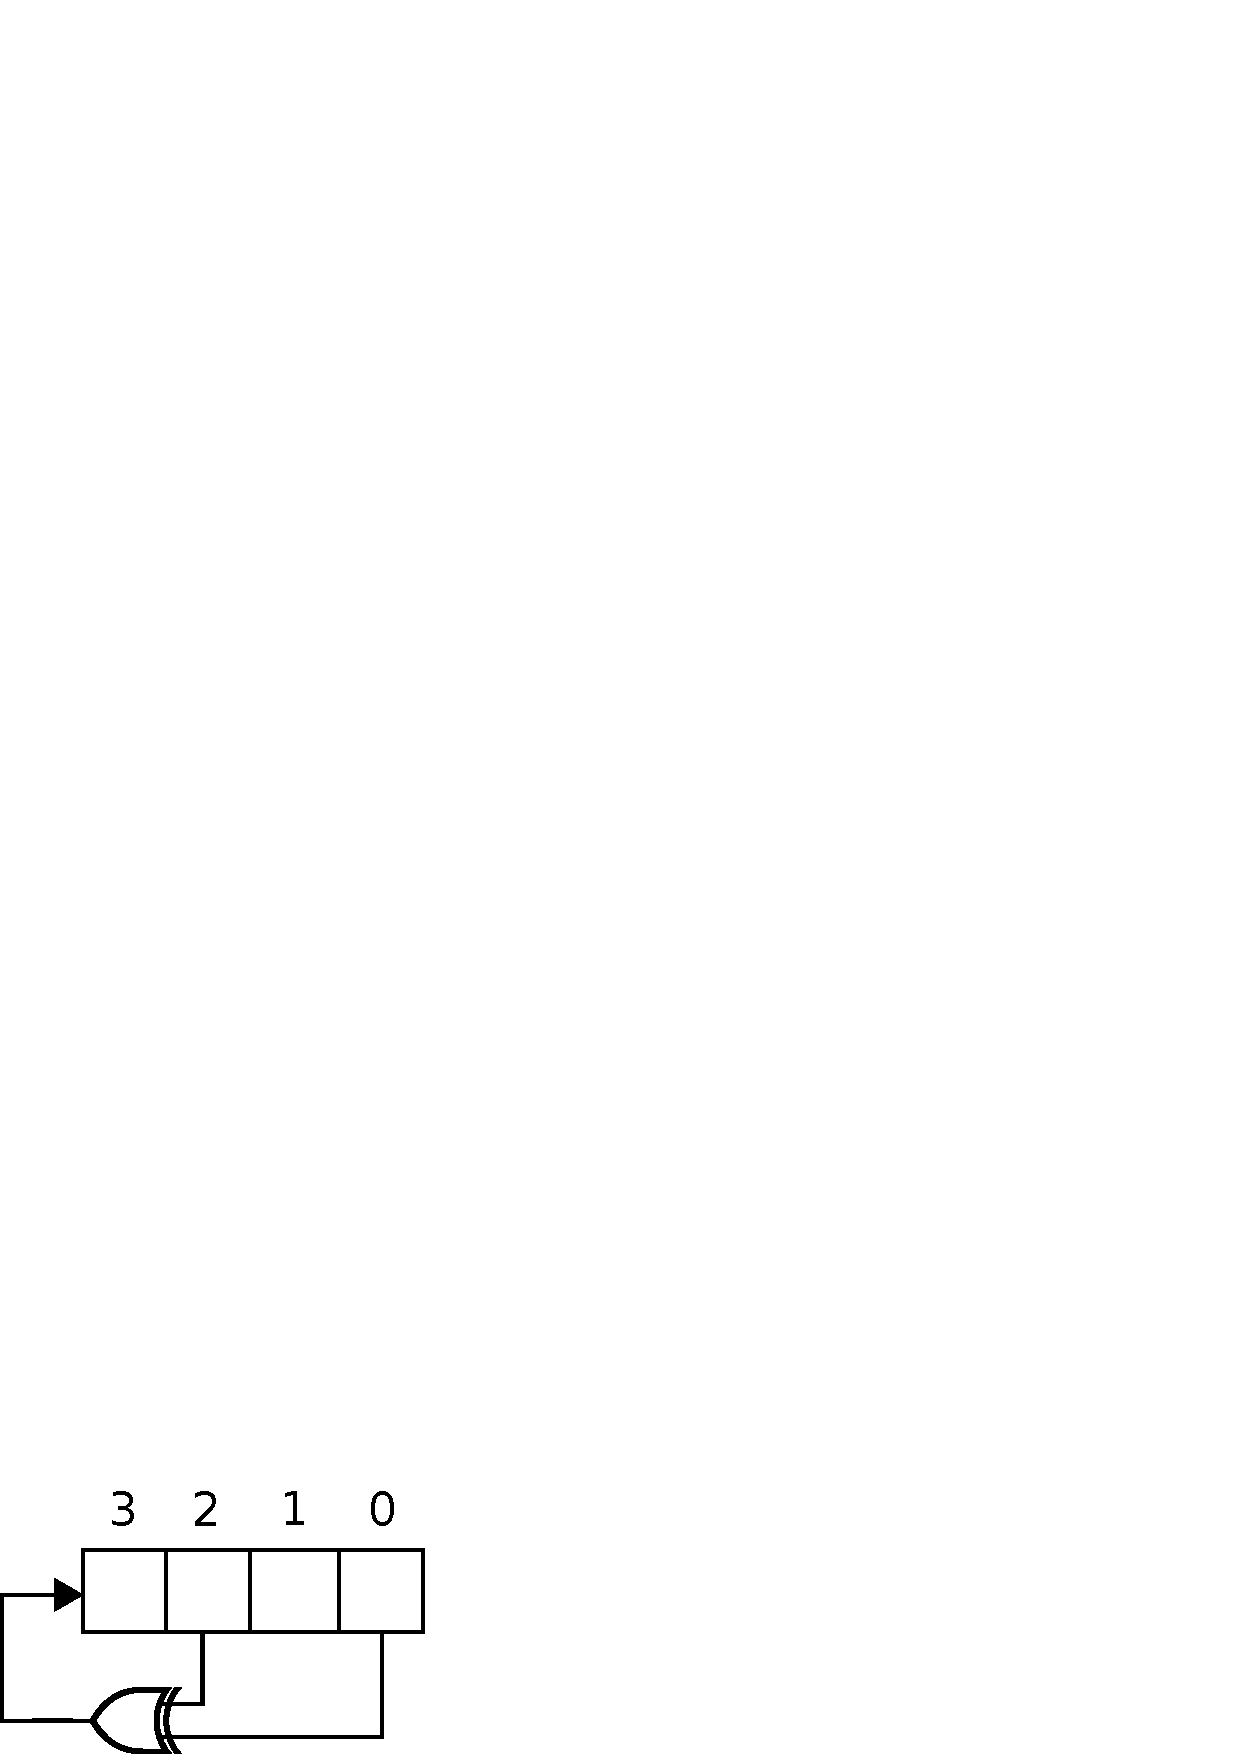
\includegraphics[width=.4\textwidth]{imgs/drawings/4bits_lfsr.pdf}
\end{figure}
This register is able to generate 6 values before it cycles back to it original state. The following listing shows all of them.\\
\par
\begin{minipage}{\textwidth}
\lstinputlisting{code/lfsr.txt}
\end{minipage}
\par
Various arrangements of taps will produce different series. In the case of this four bits register, the maximum number of values in a series is 16-1 = 15 (zero cannot be reached.) This can be achieved with taps on bits 0 and 1. This is called a "Maximum-Length" LFSR.\\
\par
\begin{minipage}{\textwidth}
\lstinputlisting{code/maximum_lfsr.txt}
\end{minipage}
\par
\par
Wolf uses a 17 bits Maximum-Length LFSR with two taps to generate a serie of pseudo-random values. Of these 17 bits, on each iteration, 9 are used to generate a Y coordinate and 8 for a X coordinate. The corresponding pixel on screen is turned red/blue.\\
\par
\begin{figure}[H] \centering \includegraphics[width=\textwidth]{imgs/drawings/fizzlefade/fibonacci.pdf} \end{figure}
\par
The above diagram is slow to implement in software. There is an alternative way to represent a LFSR called "Galois", which is the way Wolfenstein 3D implements its LFSR and writes 320x200=64000 pixels exactly once with deterministic duration.
\par
\begin{figure}[H] \centering 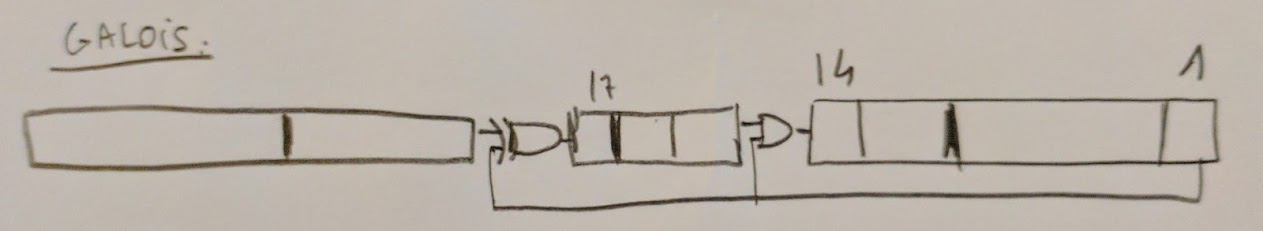
\includegraphics[width=\textwidth]{imgs/drawings/fizzlefade/galois.pdf} \end{figure}
      
\bu{Note :} Because the effect works by plotting pixels individually, it was hard to replicate when developers tried to port the game to hardware accelerated GPU. None of the ports managed to replicate the fizzlefade except Wolf4SDL, which found a LFSR taps configuration to reach resolution higher than 320x200.\\
\par
\bu{Note :} The tap configuration on 17 bits regerates 131,072 values before cycling. Since 320x200=64000, it could have been implemented with a 16 bits Maximum-length register with taps on 16,15,13 and 4 (in "Galois" notation.)










\subsection{Palette}
Even though it limited the graphic capabilities of the game, the palette system can be turned into a strength. It is easy to fade the screen to white (when picking up an item), red (when taking damage), or black (for transition between 2D menus.) It only takes 256*3 = 768 bytes and 768 out instructions to modify the full screen.
\begin{figure}[H]
  \centering
 \fullimage{palette_damage.png}
 \caption{The palette RGB colors altered when taking damage.} \label{fig:palette_damage}
\end{figure}
A fast path is provided (which ironically only works if the CPU is as slow at the VGA) to update the palette via one \cw{lobsb} instruction. Otherwise if not supported a loop of 768 \cw{outsb} is used.\\
\par
\begin{minipage}{\linewidth}
\lstinputlisting[language=C,morekeywords={asm,byte,far}]{code/vl_setpalette.c}
\end{minipage}








\section{Pseudo random generator}
Random numbers are necessary for many things during runtime. For example, to calculate if an enemy is able to hit the player based on its accuracy. This is achieved with a precalculated pseudo-random series of 256 elements. The last random value is also the index of the next value.\\
\par
\begin{minipage}{\textwidth}
\lstinputlisting[language={[x86masm]Assembler}, style=mystyle,basicstyle=\small]{code/rndtable.asm}
\end{minipage}
\par
The pseudo-random series is initialized using the current time modulo 256 as seen.\\
\par

\begin{fancyquotes}
The random table wasn't even a shuffle - note that there are no 1s and two 2s in the table. I built it by just storing out 256 randoms from a little C program.  This was bad!
\bigskip \\
\textbf{John Carmack - Programmer}
 \end{fancyquotes}

\par
\begin{minipage}{\textwidth}
\lstinputlisting[language={[x86masm]Assembler}]{code/US_InitRndT.asm}
\end{minipage}
\par
The random number generator saves the last index in \cw{rndindex}. Upon request for a new number, it simply looks up the new value and updates \cw{rndindex}.
\par
\begin{minipage}{\textwidth}
\lstinputlisting[ language={[x86masm]Assembler}]{code/US_RndT.asm}
\end{minipage}

This pseudo random serie of 256 values could have been generated with an 8 bits Maximun length LFSR (8,6,5,4). My assumption is that LFSR literrature was hard to find at the time and finding the correct tap for a maximum length register of 16 bits was not worth the effort.\\







